% Copyright © 2015-2016 Martin Ueding <dev@martin-ueding.de>
%
\documentclass[english, fleqn]{beamer}

\usetheme{Malmoe}
%\usetheme{Dresden}
%\usetheme{Marburg}

\usepackage[bibatend, beamer]{../../header}
\usepackage{adjustbox}
\usepackage{transparent}

\renewcommand\iup{\text i}
\renewcommand\eup{\text e}

\graphicspath{{./}{../Figures/}}

\title{Positron lifetime in metals and insulators}
\subtitle{Experiment K225 -- Universität Bonn}
\author{%
    Martin Ueding
    \and
    Lino Lemmer
}
\date{\daterange{2016-03-24}{2016-03-25}}

\newcommand\transition[2]{%
    {
        \setbeamertemplate{background canvas}{%
            \includegraphics[height=\paperheight]{#2}
        }
        \begin{frame}[plain]
            \centering
            \transparent{0.8}
            \colorbox{white}{%
                \marginbox{1ex}{%
                    \begin{huge}
                        #1
                    \end{huge}
                }
            }
        \end{frame}
    }
}

\newcommand\oscillatorSize{0.7}

\begin{document}

\begin{frame}
    \titlepage
\end{frame}

\section{Theory}

\subsection{Positron sources}

\begin{frame}
\includegraphics{beamer-na22}
\end{frame}

\begin{frame}
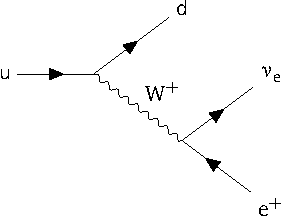
\includegraphics{beamer-beta}
\end{frame}

\subsection{Positron decay}

\begin{frame}
    \frametitle{Decay modes of positrons}

    \begin{columns}[c]
        \begin{column}{.5\textwidth}
            \centering
            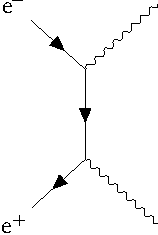
\includegraphics{beamer-two-photon}
        \end{column}
        \begin{column}{.5\textwidth}
            \centering
            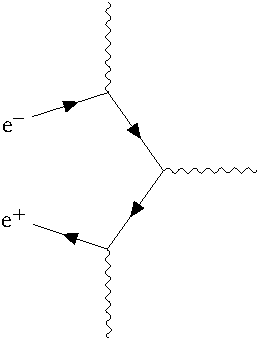
\includegraphics{beamer-three-photon}
        \end{column}
    \end{columns}
\end{frame}

\subsection{Detector and electronics}

\begin{frame}
    \includegraphics{beamer-scheme-176Lu}
\end{frame}

\begin{frame}
    \includegraphics{beamer-photomultiplier}
\end{frame}

\begin{frame}
    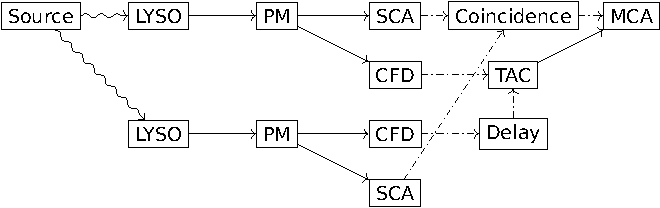
\includegraphics{beamer-fast-slow}
\end{frame}

\subsection{Bootstrap}

\transition{Bootstrap}{boots-3}

\section{Conduction}

\transition{Conduction}{rack-and-detector}

\subsection{Slow circuit setup}

\begin{frame}
    \includegraphics{beamer-lyso-li}
\end{frame}

\begin{frame}
    \includegraphics{beamer-lyso-re}
\end{frame}

\begin{frame}
    \includegraphics{beamer-na-li}
\end{frame}

\begin{frame}
    \includegraphics{beamer-na-re}
\end{frame}

\begin{frame}
    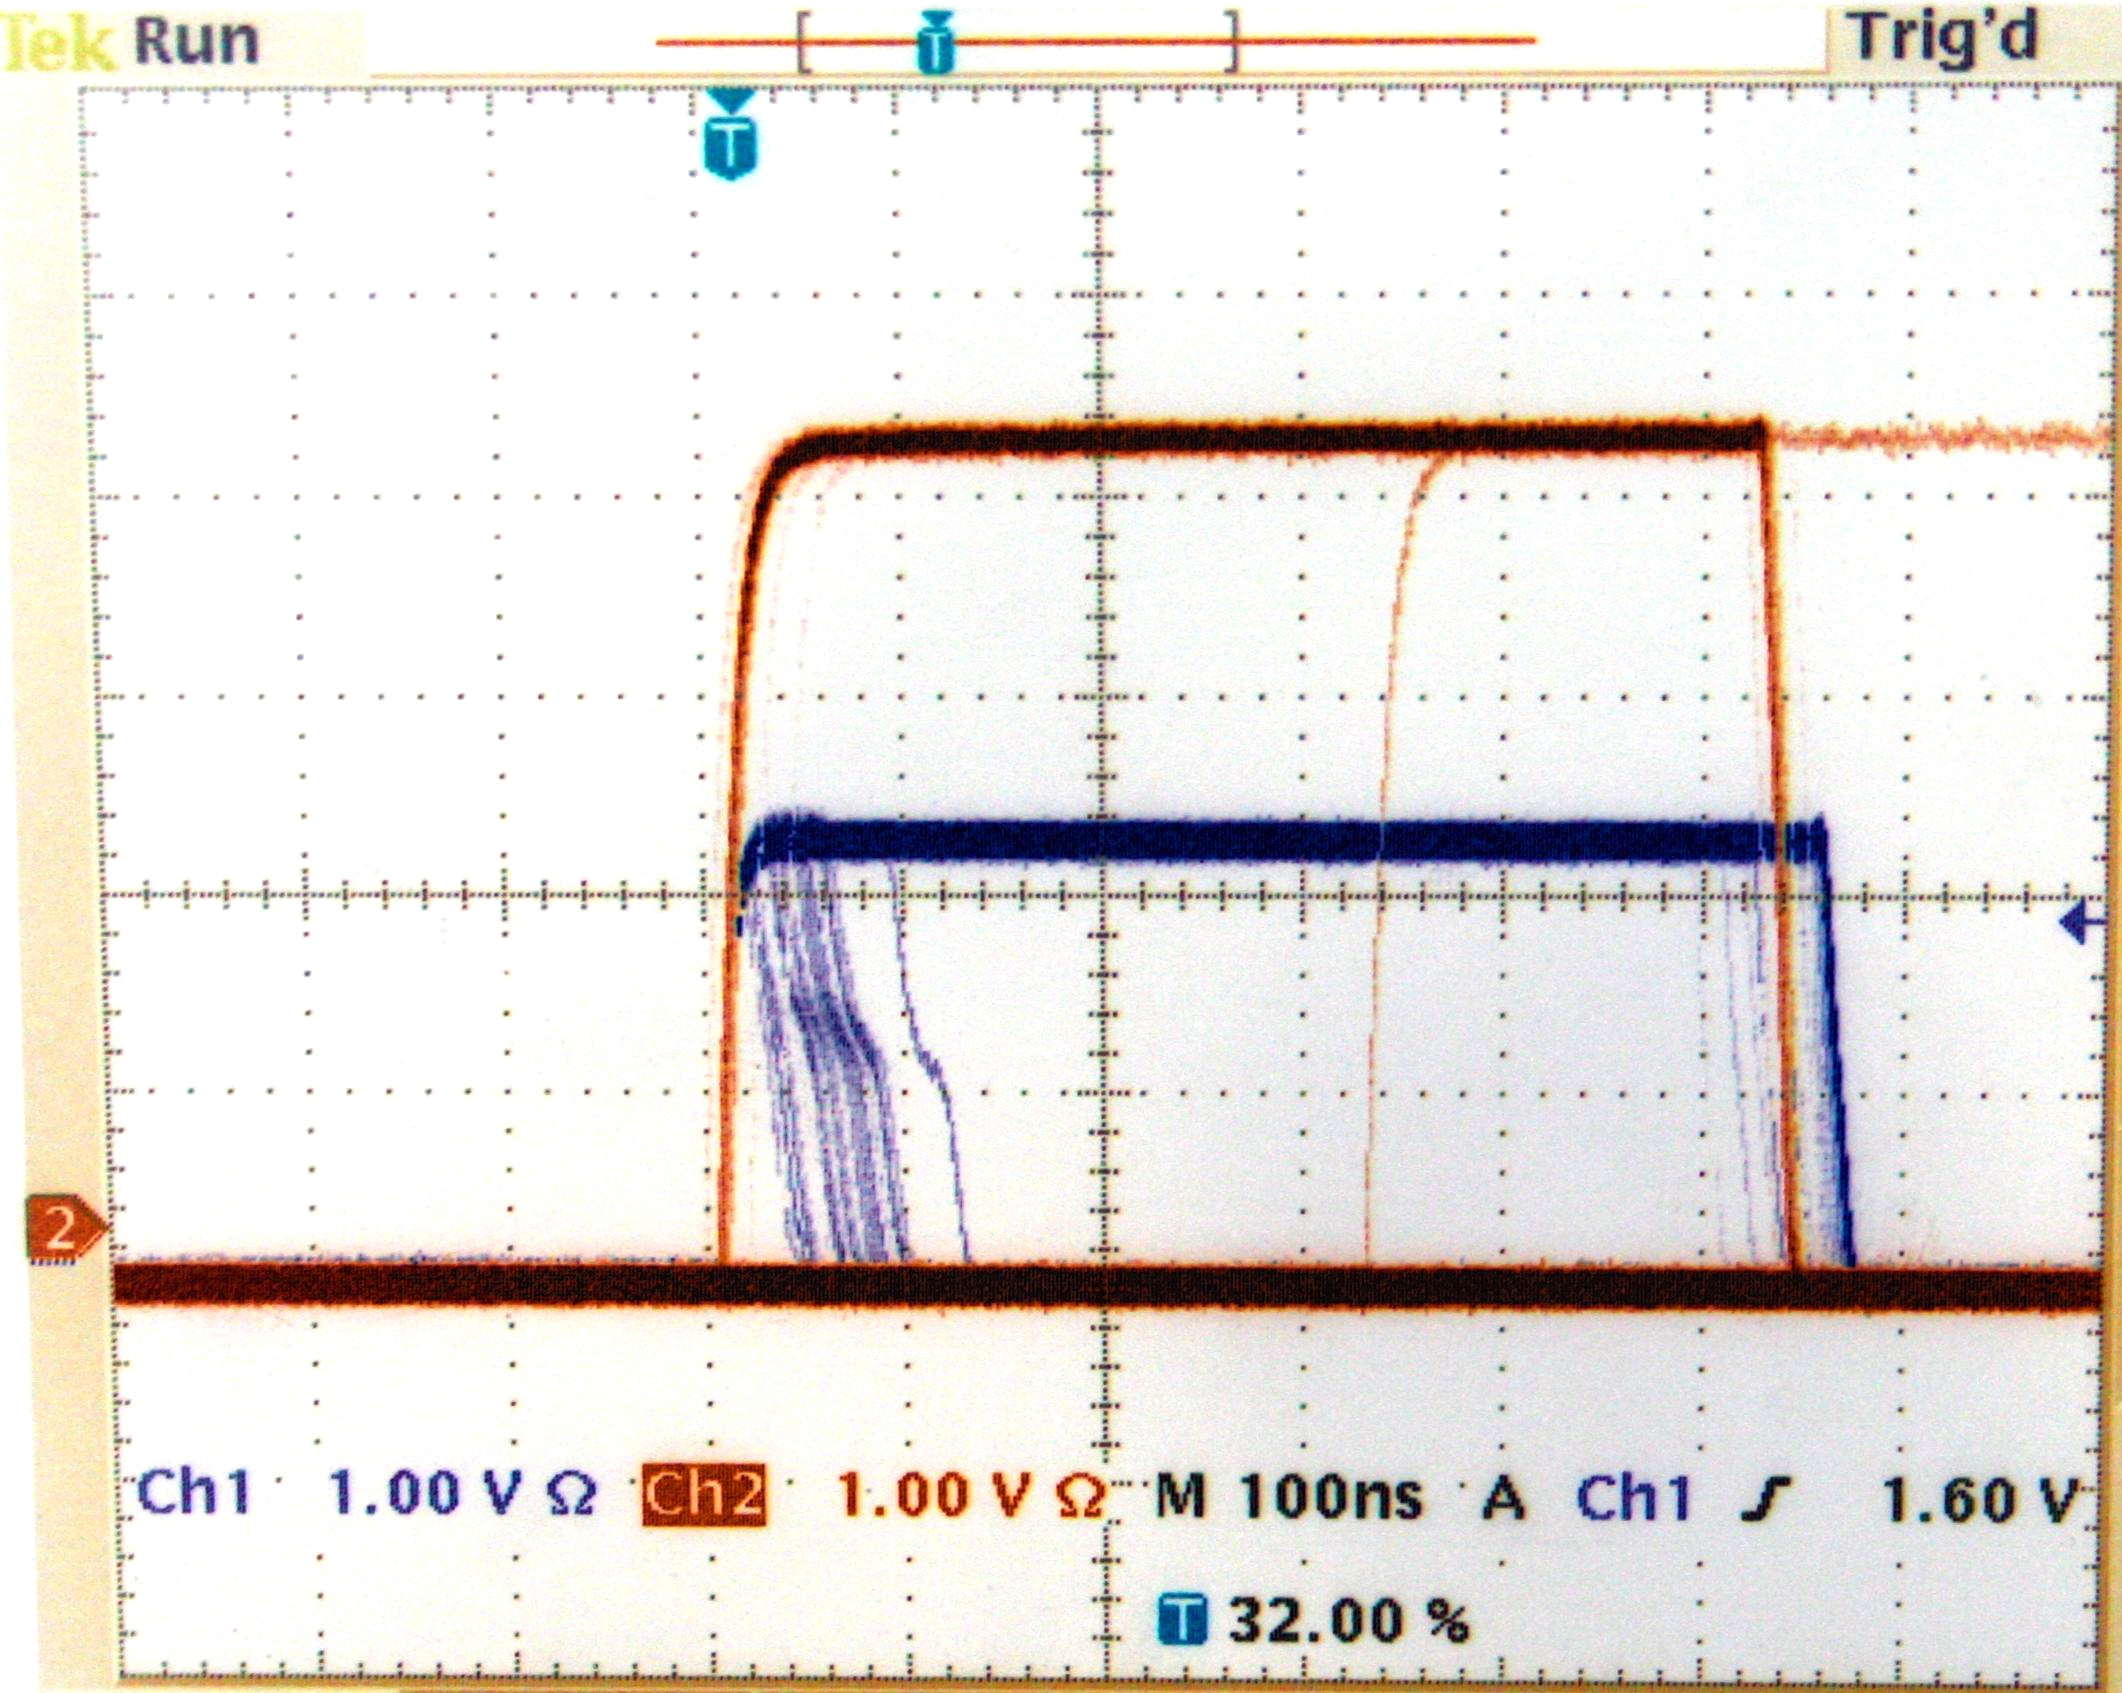
\includegraphics[height=\oscillatorSize\textheight]{br-1-sca-coincidence-511}
\end{frame}

\begin{frame}
    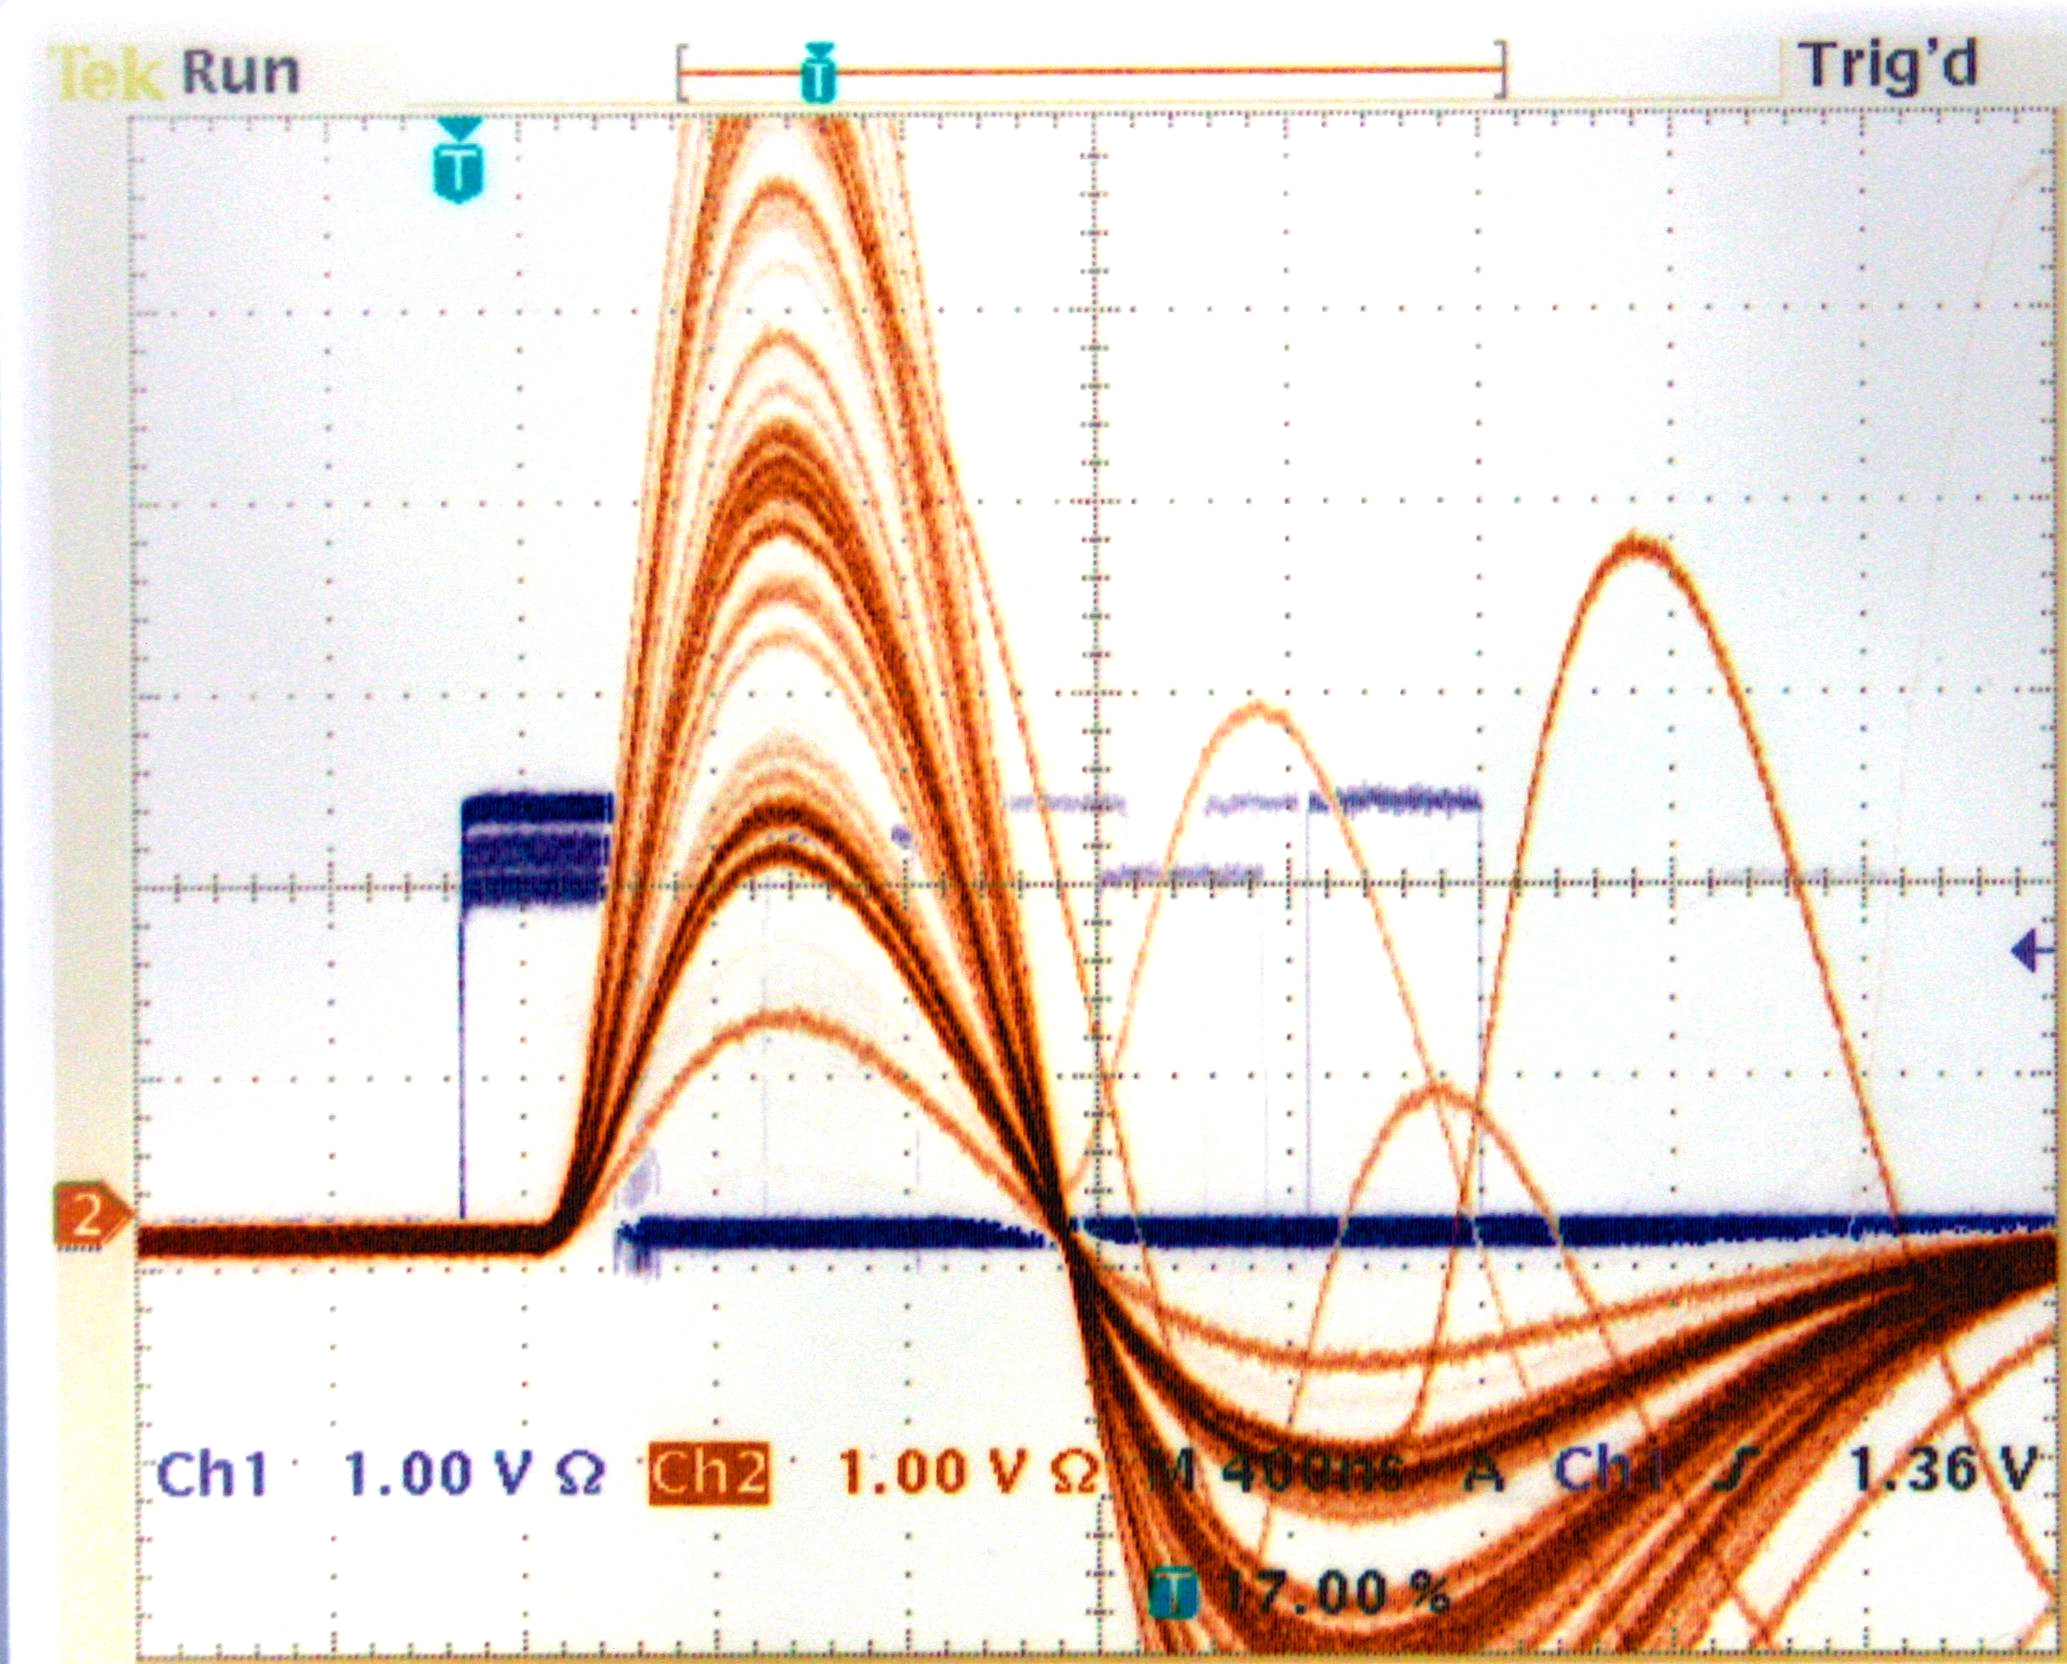
\includegraphics[height=\oscillatorSize\textheight]{br-2-sca-and-slow}
\end{frame}

\subsection{Fast circuit setup}

\begin{frame}
    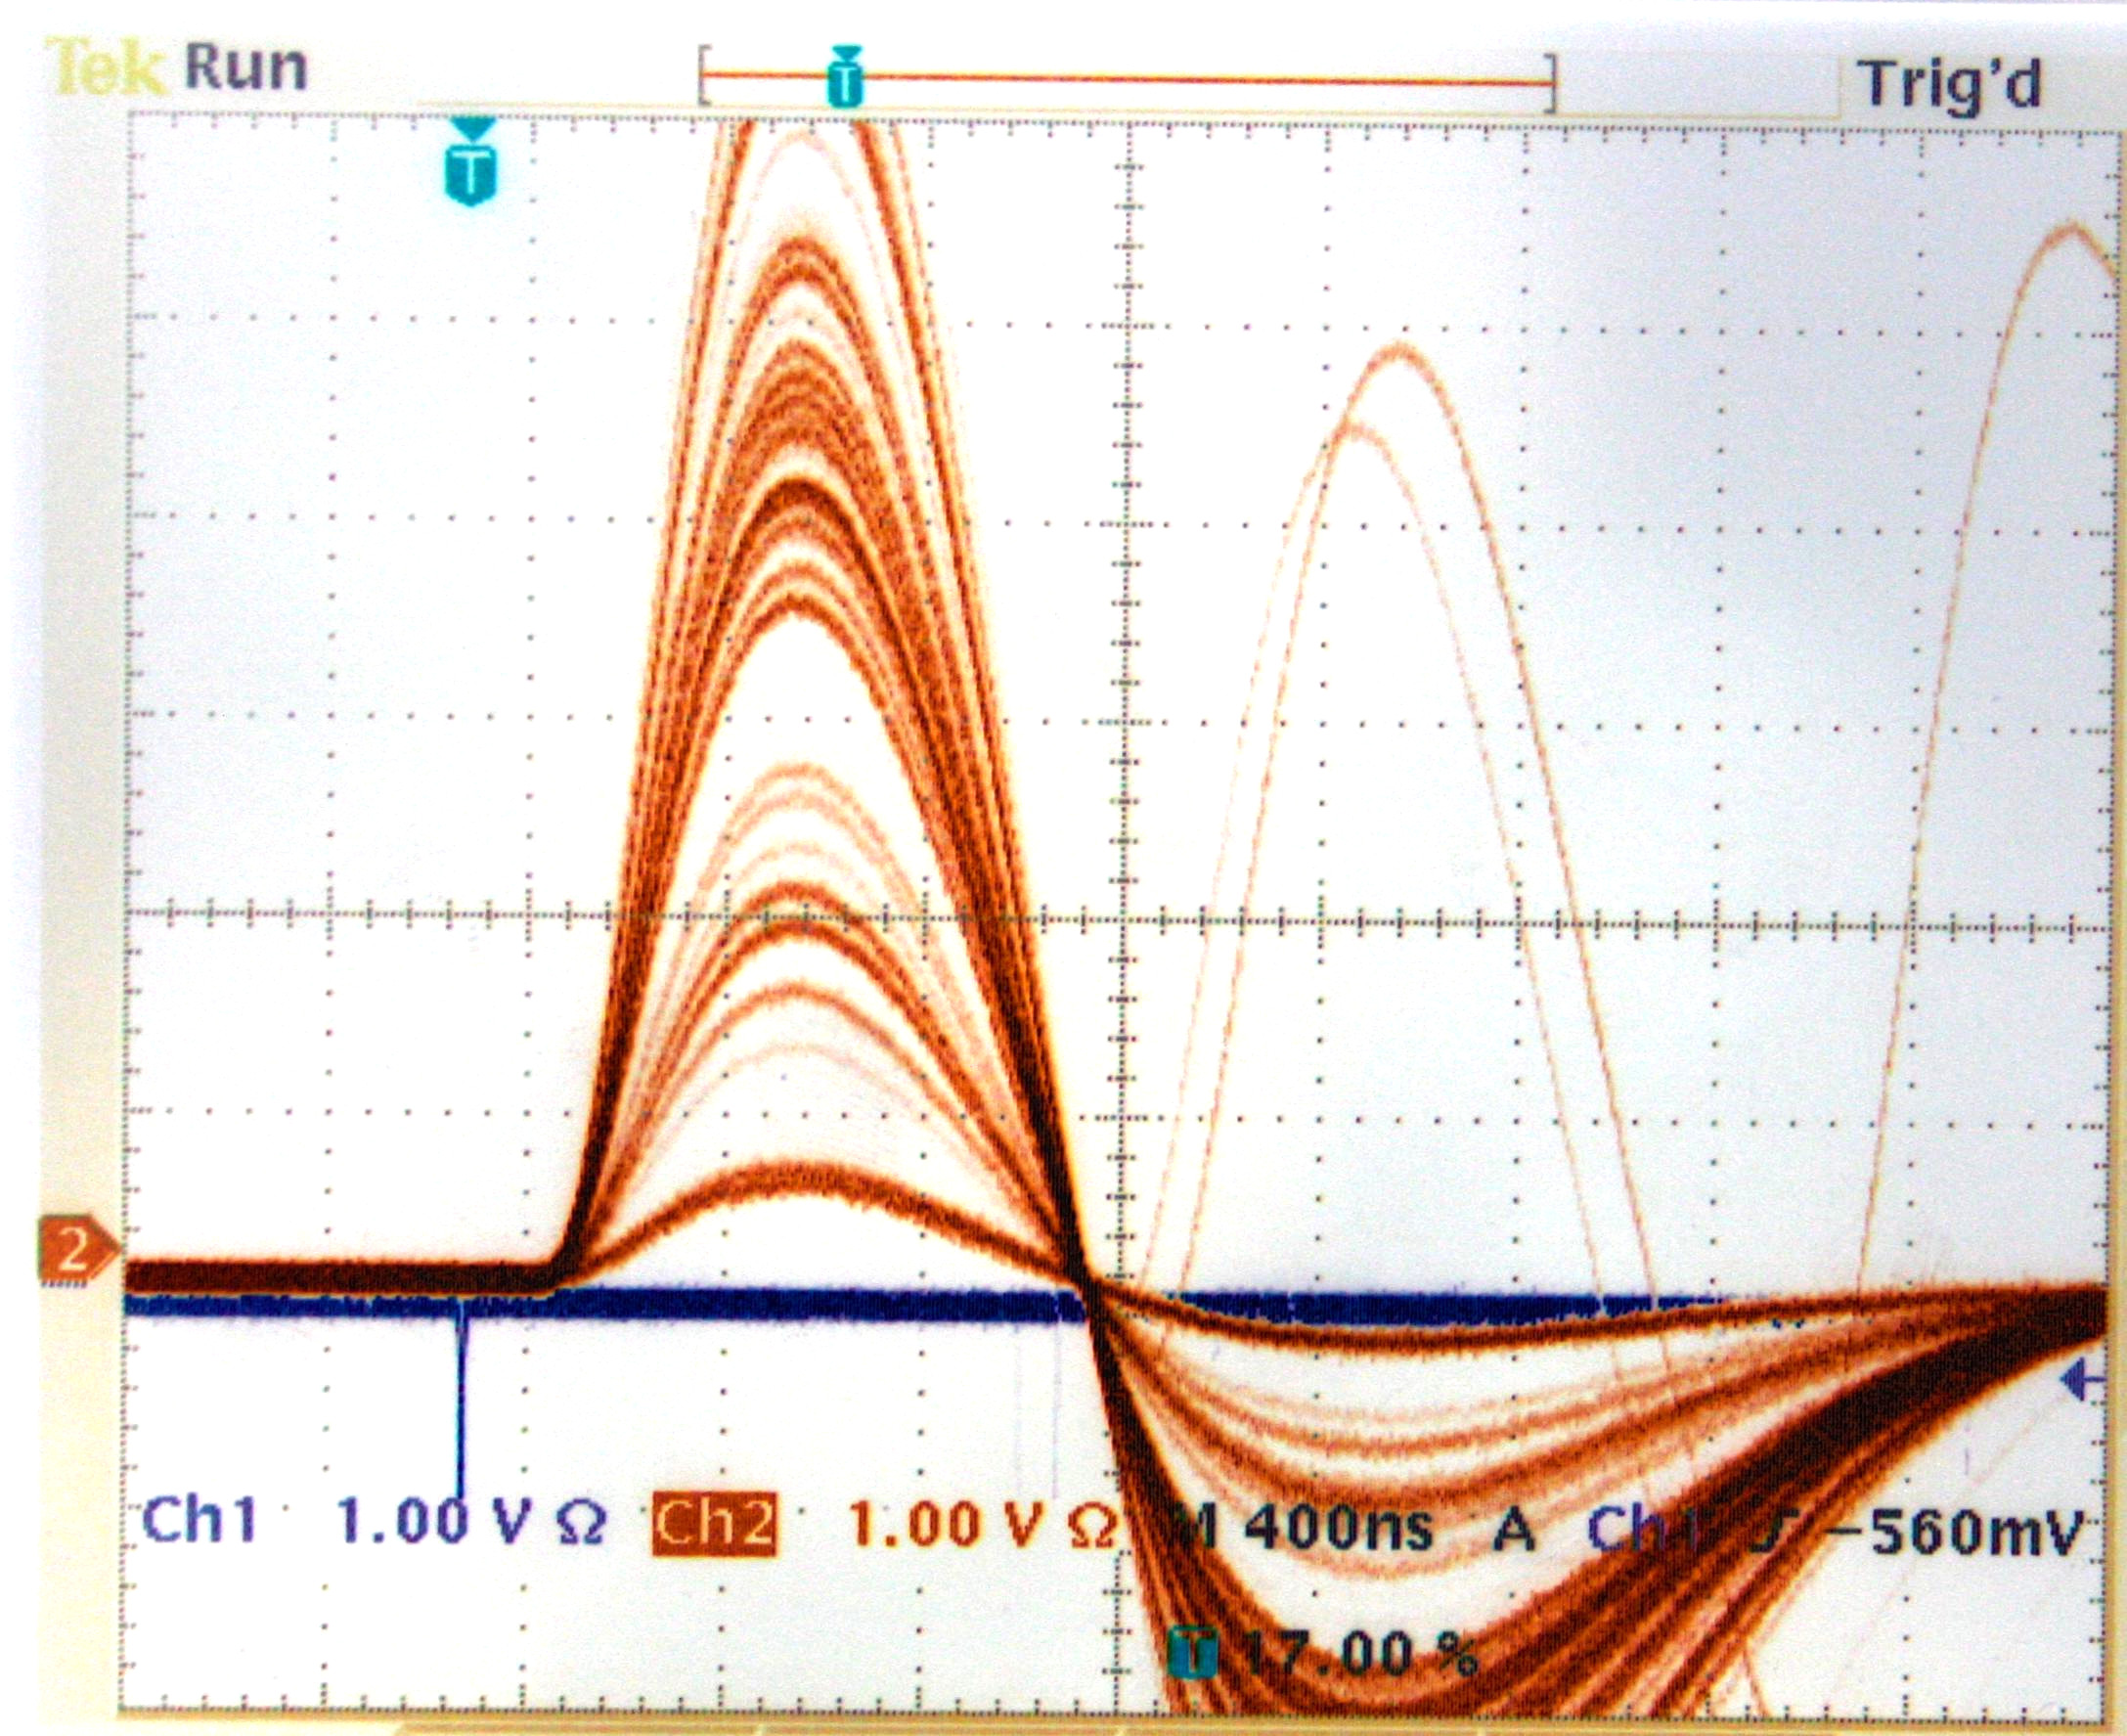
\includegraphics[height=\oscillatorSize\textheight]{br-3-cfd-and-slow}
\end{frame}

\begin{frame}
    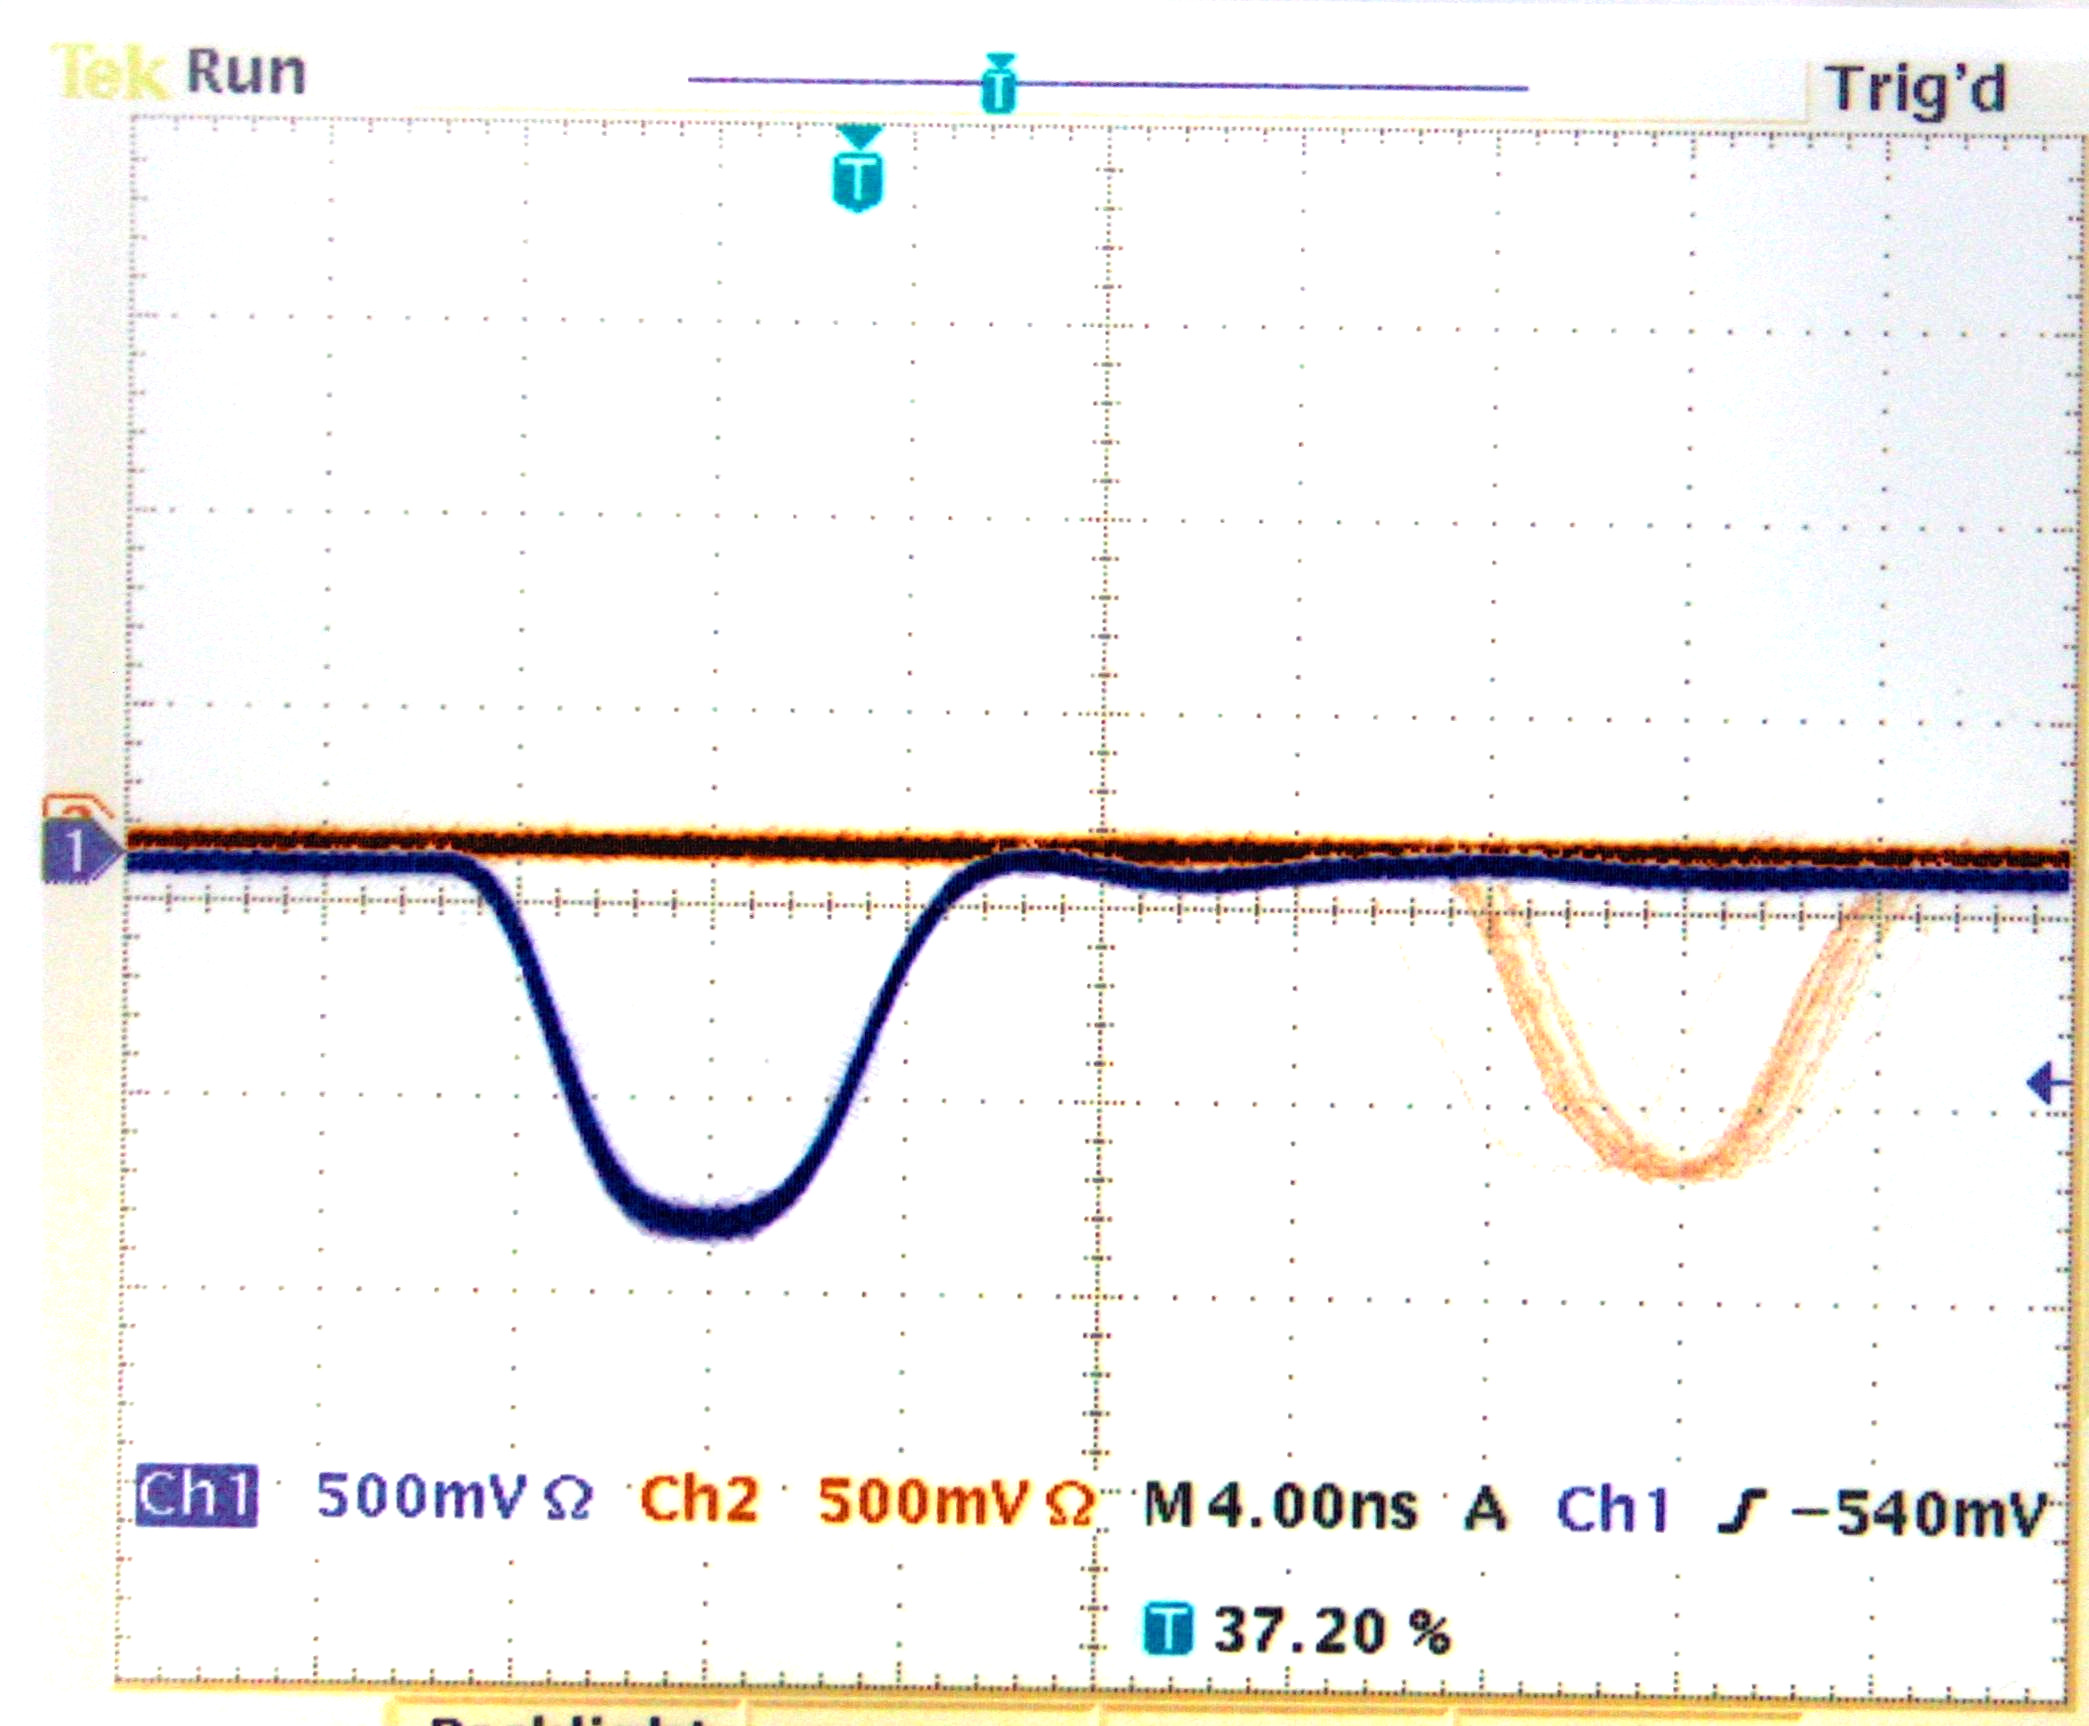
\includegraphics[height=\oscillatorSize\textheight]{br-4-cfd-delay}
\end{frame}

\subsection{Time calibration}

\begin{frame}
    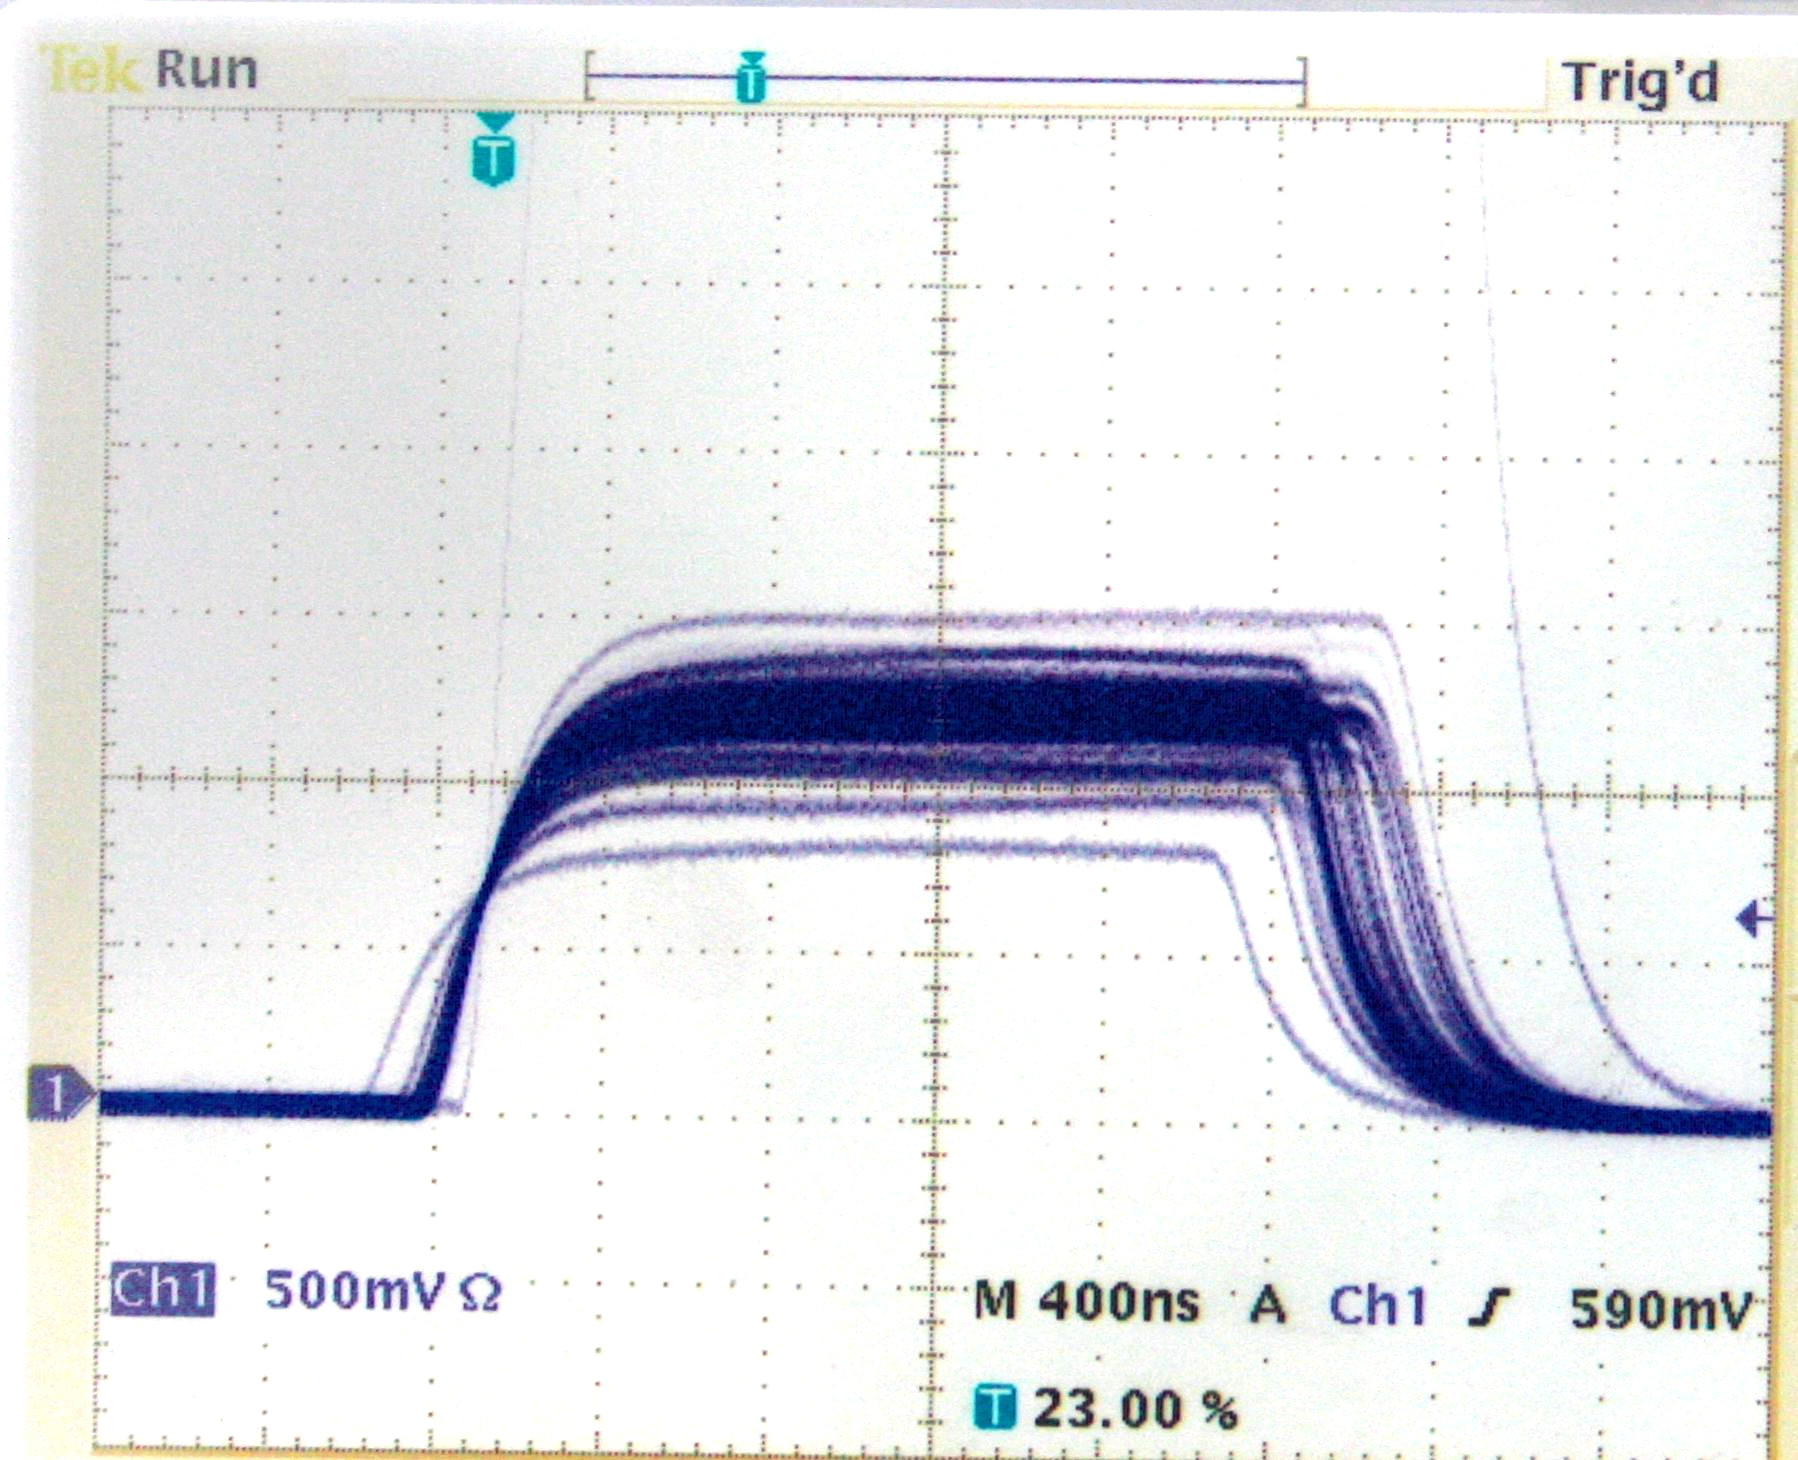
\includegraphics[height=\oscillatorSize\textheight]{br-5-tac-511}
\end{frame}

\begin{frame}
    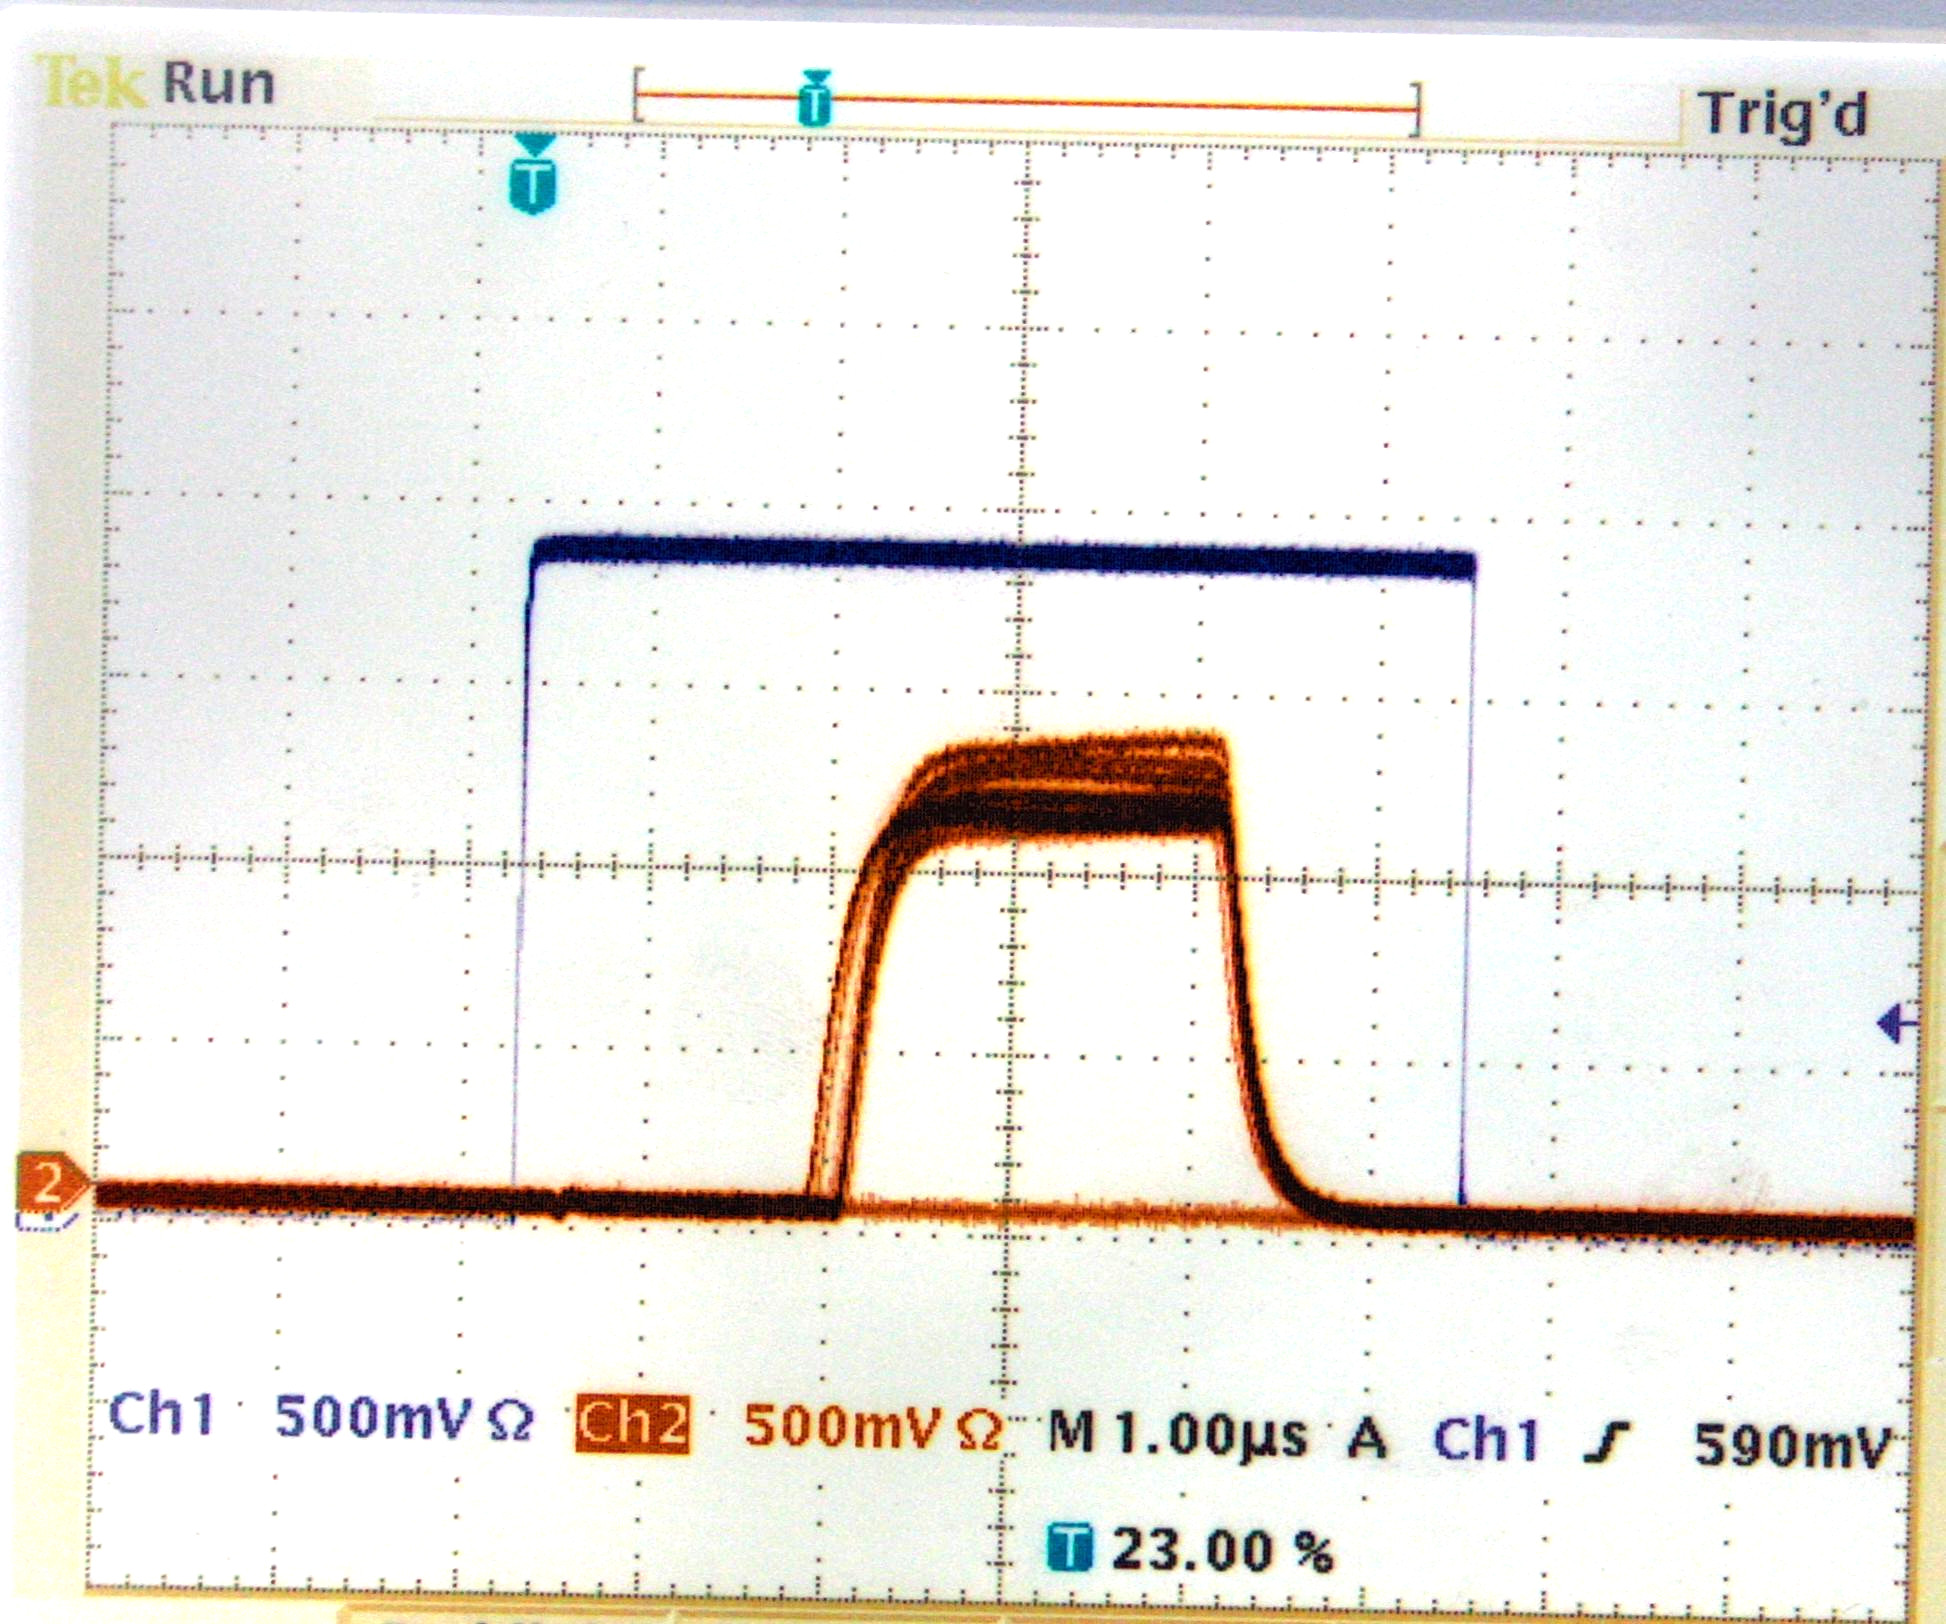
\includegraphics[height=\oscillatorSize\textheight]{br-6-tac-and-coincidence-511}
\end{frame}

\begin{frame}
    \includegraphics{beamer-prompts_short}
\end{frame}

\begin{frame}
    \includegraphics{beamer-prompts_long}
\end{frame}

\begin{frame}
    \includegraphics{beamer-time_gauge}
\end{frame}

\begin{frame}
    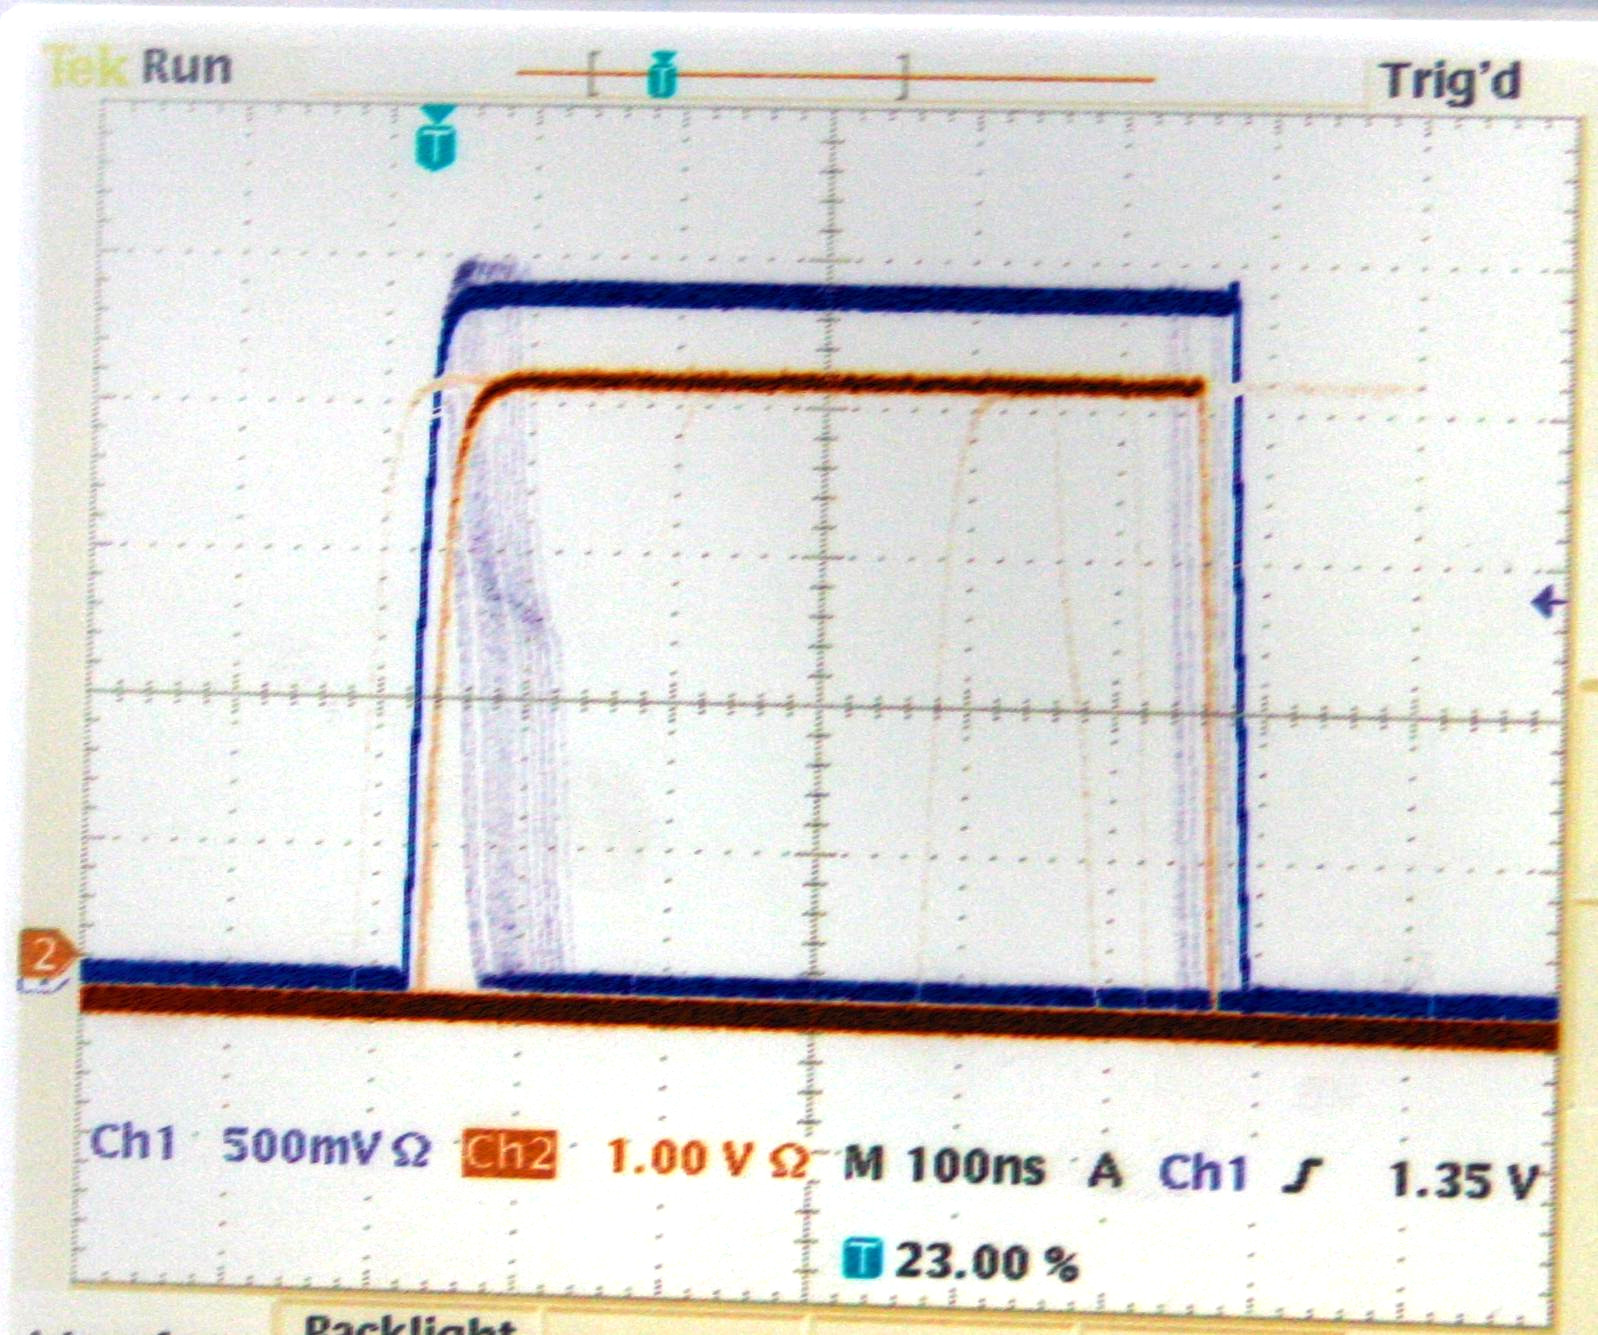
\includegraphics[height=\oscillatorSize\textheight]{br-7-sca-coincidence-1275}
\end{frame}

\begin{frame}
    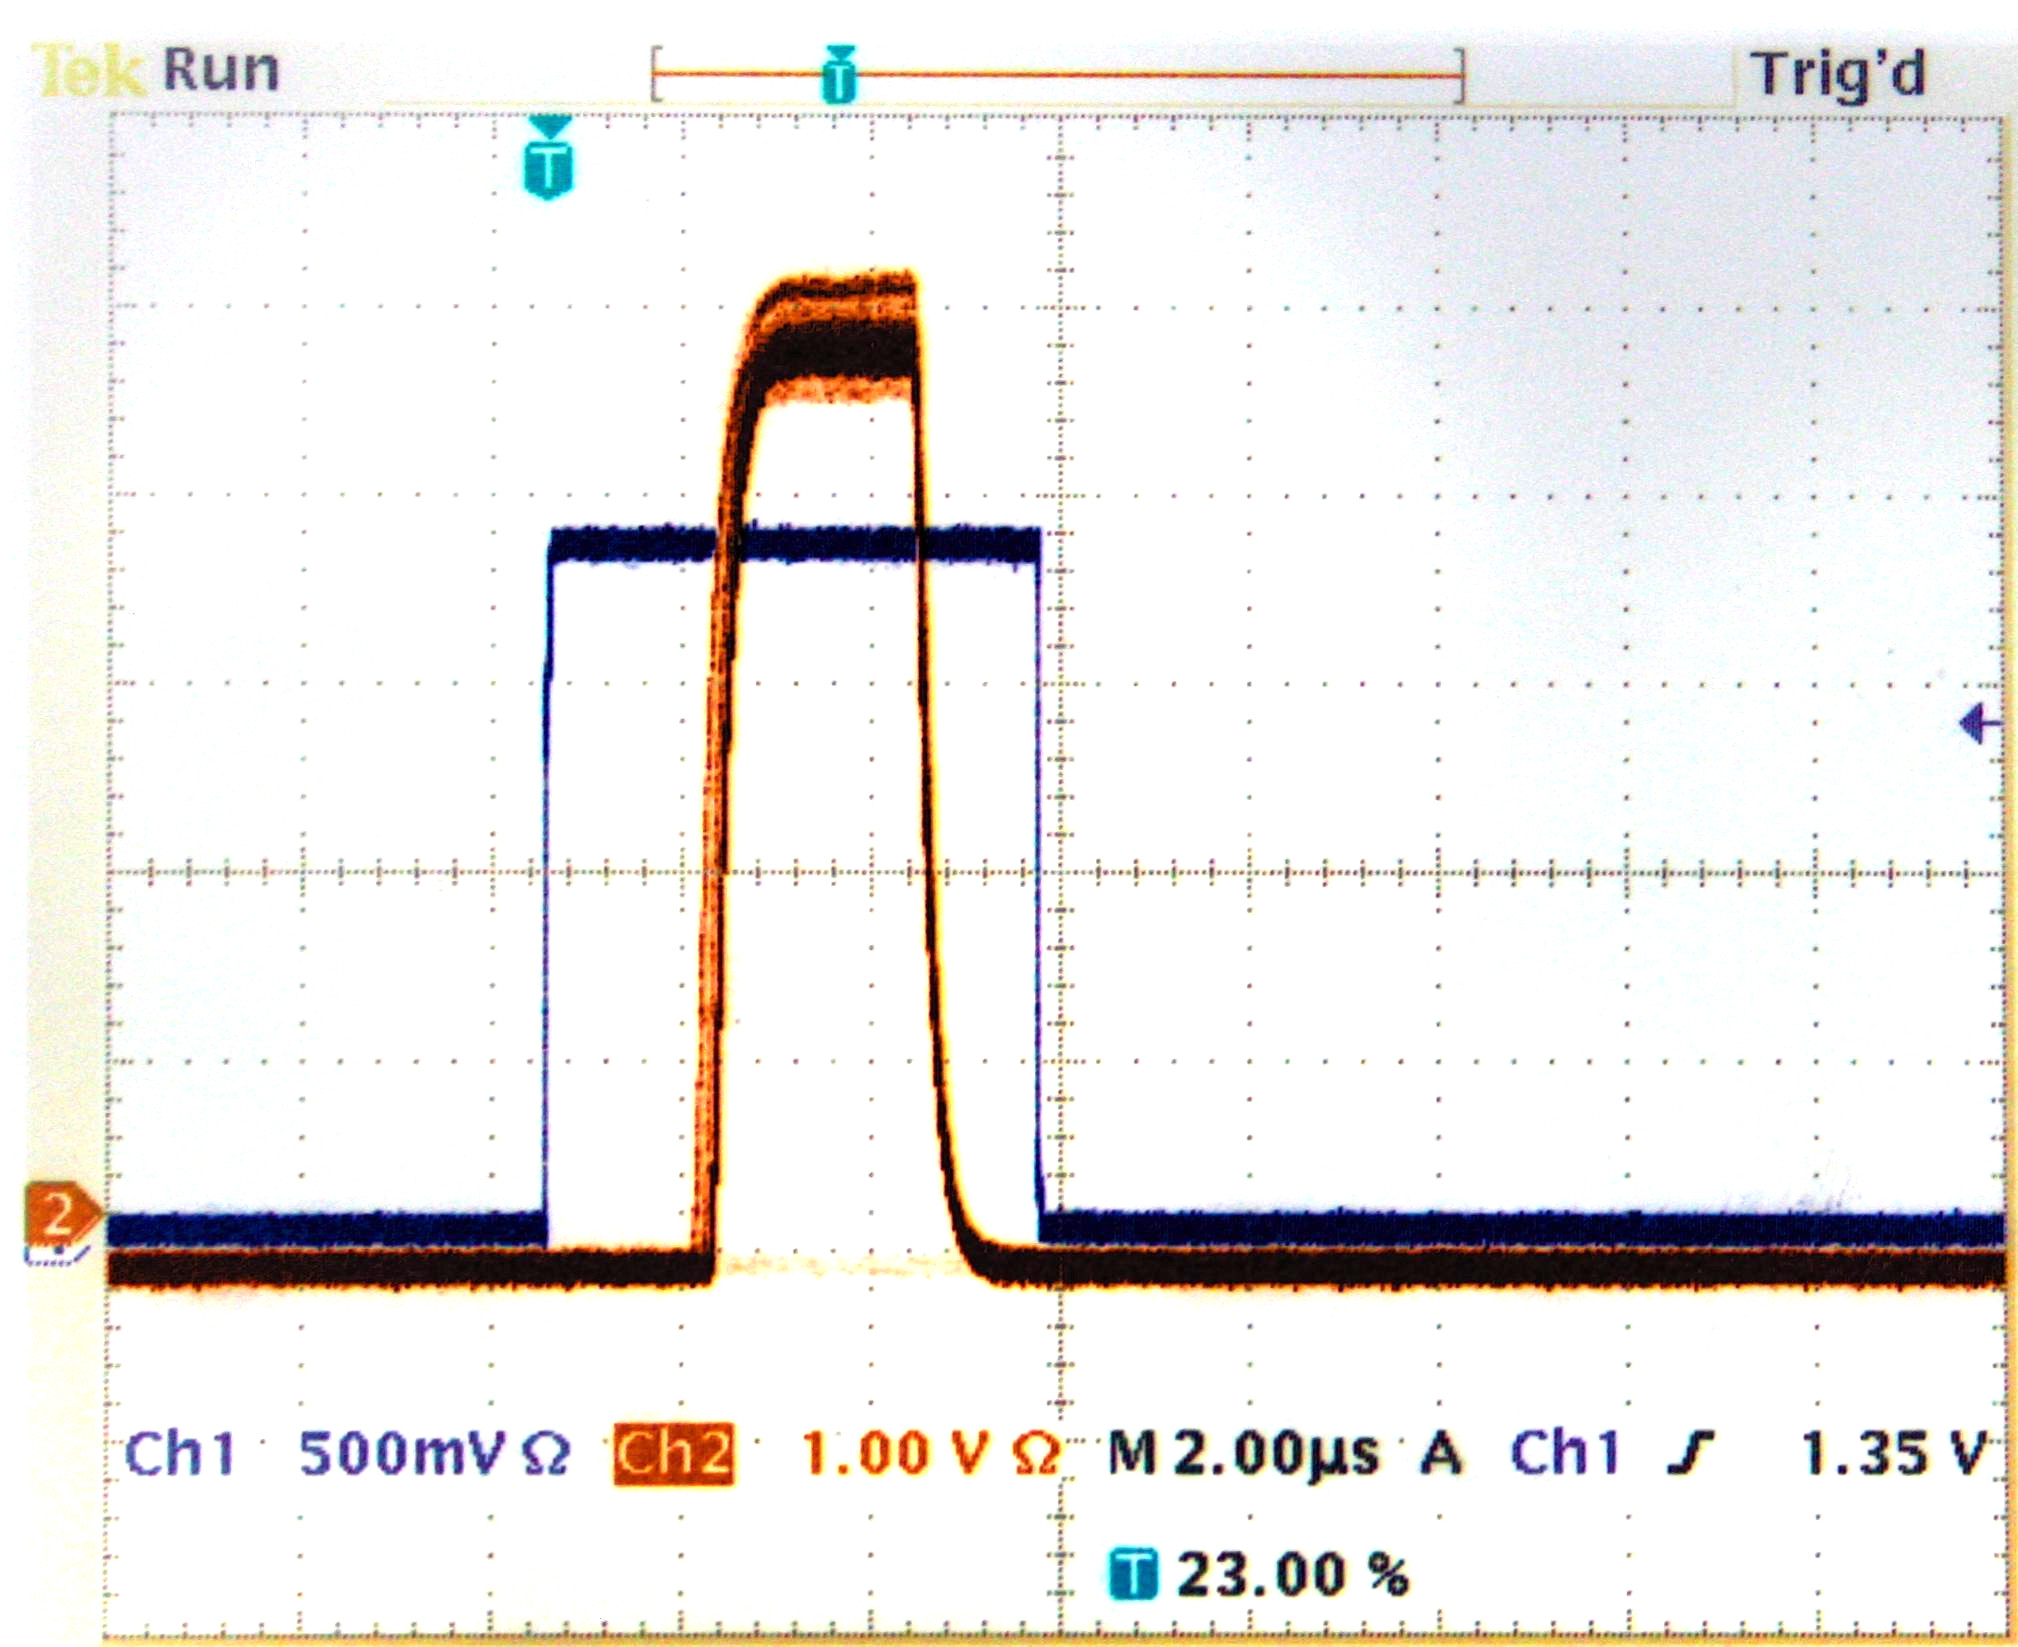
\includegraphics[height=\oscillatorSize\textheight]{br-8-tac-and-coincidence-1275}
\end{frame}

\subsection{Lifetime measurement}

\begin{frame}
    \includegraphics{beamer-lifetime-295K}
\end{frame}

\section{Analysis}

\transition{Analysis}{crunch1}

\subsection{Lifetimes}

\begin{frame}
    \includegraphics{beamer-taus}
\end{frame}

\begin{frame}
    \includegraphics{beamer-intensities}
\end{frame}

\subsection{Vacancy formation enthalpy}

\begin{frame}
    \includegraphics{beamer-s_curve}
\end{frame}

\begin{frame}
    \frametitle{Arrhenius plot}

    \includegraphics{beamer-arrhenius}
\end{frame}

\begin{frame}
    \includegraphics{beamer-acrylic}
\end{frame}

\subsection{Acyclic glass}

\begin{frame}
    \includegraphics{beamer-acrylic-zoom}
\end{frame}

        %\includegraphics{lifetime-<< temp >>K}

\begin{frame}
    \frametitle{References}

    \printbibliography
\end{frame}

\end{document}

% vim: spell spelllang=en_us
